\chapter{Problem Domain}\label{part:analysis}

In this chapter, we will expand on our view of the problem domain of simulations, in order to better provide an understanding of our intentions with The Language Described in this Report, and the basis upon which we argue. The chapter will briefly cover reasons for modelling and different approaches to modelling. Following this is a section on simulations in general, and specific ways of doing theoretical simulations. This also addresses some problems with the creation of computer simulations, and how such a problem can be viewed.

\section{Models}
Model is a term often used in both natural and social sciences. Unfortunately the term is not as well defined as it perhaps should be, and it will therefore here be specified what is meant by it. The approach here is based on Mario Bunge definition of a model. According to his theory a model consists of two parts:
\begin{itemize}
\item A general theory
\item A special description of an object or system (model object)
\end{itemize}
This perception is a very general way of thinking of models and often works very well with natural and, to some degree, social  sciences where experiments and models are based on an overall theory and consists of objects and systems. In social sciences, though, it often happens that the general theory is vaguely defined og even non-existant and the purpose of the model is only to observe interactions and behaviour of the systems and their objects.
To extend Bunges theory models will here be defined as \enquote{a set of assumptions about some system} meaning everything we know about a system that we can observe or a theoretical system.
Genrally there are two different types of models, static and dynamic models.

\subsection{Dynamic Models}
Dynamic models includes some form of evolution, meaning that the system changes due to some changing factor. This is often time, but can also be things like energy, as is often the case in chemistry, or alike, the only important thing is that the factor changes. Nearly all systems in natural and social sciences are dynamic models.

\subsection{Static Models}
A static model is a snapshot of a given system with objects with non-changing states. These systems are often not very representative for reality since nearly all systems changes but they can still be very usefull to construct since it can be much easier to collect information and understanding through a static model. 

\section{Simulation}
We often need to create and analyse models. For a portion of these models an analytical approach can be used, where the one can analyse the model via mathematical methods and calculate how static models will look and dynamic models evolve. This approach only works on a limited portion of the models where the system and behaviour of objects are well known and can be described mathematically. As the models become more stochastic purely mathematical analysis begins to fall short and simulations are often used to be able to create the (often dynamic) models.

Formally simulations is defined as \enquote{a system designed to imitate another real system} \jenote{Find a better definition of a simulation}. This is a very broad definition, since real systems can be very different in their structure and further more the type of simulations also differs greatly. Generally one can distinguish between two different types of simulations, experimental and theoretical. An experimental simulation is where a real system is imitated by another real system, often smaller and/or simpler. For instance when biologists simulate the creation of life on the back of crystals in their lab it is an experimental simulation. Theoretical simulations are simulations where a real system is imitated theoretically often on a computer or on paper. This project will focus on theoretical simulations. To further narrow the definition of a simulation used in this project, the focus will mainly be put on natural and social sciences where simulations are most often used. Within these sciences real systems can still vary a lot, but they nearly always share the property that they change state over, what is often but not necessarily, time. This is close to the definition of a dynamic model. In this respect simulations are close to a dynamic model.
How this change is modelled can also vary and generally we often speak of two different paradigms; Discrete and continuous simulations.

\subsection{Discrete Simulations}
Discrete simulations are often dictated by flows and states where the state of the whole system and subsystems are updated in discrete iterations. The systems and objects update their state each iteration. Observations in discrete simulations does not make sense during update but only before/after iterations. Figure \jenote{Make figure} shows an illustration of discrete simulations. Here we can see that the model updates instantaneous between iterations. This abstractions tend to be more useful when the simulations are better known and knowledge exists on how iterations are set in motion and the state is updated.

\subsection{Continuous Simulations}
Continuous simulations are simulations that can be described with differential change. This means that 

% We make for ourselves internal images or symbols of the external objects, and we make them in such a way that the consequences of the images that are necessary in thought are always images of the consequences of the depicted objects that are necessary in nature ... Once we have succeeded in deriving from accumulated previous experience images with the required property, we can quickly develop from them, as if from models, the consequences that in the external world will occur only over an extended period or as a result of our own intervention.
\label{simulationchoise}
As an abstraction for the language to create simulations

\subsection{The Iteration Problem}
By choosing the actor model it is, as explained in \cref{simulationchoise}, possible to create continuous simulations in the language with a good abstraction for simulations and models in general. Unfortunately the actor model does not support discrete simulations very well and when trying to create discrete simulations with this one deep problem arises that needs to be addressed.
The problem is that there is no way for the programmer in the language to tell whether a group of actors has stopped working or not. This is important since the user must to be able to implement iteration steps if he or she is to create discrete simulations. He or she has to be able to find out when one step has ended to update the state of the whole system and start a new iteration. Due to the parallel nature of the actor model an unfortunate variant of race conditions arise.
For an actor to have stopped the programmer needs to know the three following:
\begin{itemize}
\item The actor is not currently executing any messages
\item The actors message queue is empty
\item The actor will not receive any further messages
\end{itemize}
The two first conditions are inherently easy to check. But for the last condition to hold one must make sure that all other actors that know about this actor also have stopped for else they can send messages to the actor and thereby \enquote{reviving} it. First of all the programmer must be able to group actors together thereby making sure that only actors in these groups can communicate with each other. This is done so he or she can know what actors must have stopped.

In this project the scope of parallelisation is within simulations. The rest of this section will describe some general properties and processes of computer simulations. At last this section will discuss generalisations and assumptions, that can be made on the basis of the understading of the problem domain. This can be used to provide the design phase with some ideas of abstractions the language should implement.

\emph{Understanding the problem domain}

Firstly before spending time in an attempt to develop a parallel solution for any problem, one should first determine whether or not the problem is one that can actually be parallelized. This will be described in \cref{top}.

\emph{Granuality}

In order to do a computable simulation of a problem, a level of granuality is to be determined, this is a significant for both computation time and accuracy of the simuilation. A description of this process is giving in \cref{dis}

\emph{Helping processes and tools for making solutions parallel}

Designing and developing parallel programs is characteristically a very manual process. The programmer is typically responsible for both identifying and actually implementing parallelism.

Manually developing parallel solutions is a time consuming, complex, error-prone and an iterative process.

Various tools can assist the programmer with converting serial programs into parallel programs. The most common type of tool used to automatically parallelize a serial program is a parallelizing compiler or pre-processor.

This is usually a process of the compiler analysing the source code of a serial solution and identifying opportunities for parallelism. The analysis includes identifying inhibitors to parallelism and possibly a cost weighting on whether or not the parallelism would actually improve performance. For example loops (do, for) are the most frequent subject to automatic parallelization.


\chapter{Solution Domain}\kanote{dette virker til at være en dårlig navngivning}\label{part:analysis2}

In this chapter, we will examine certain technological tools for handling problems within the domain of computer simulations. This will include a section on High Performance Computing (HPC), which is the way to do simulations, and how this is done today. Right after the HPC section, a section on parallelism, based on theory from computer science. This section on parallelism covers the attractiveness of parallelism, as well as the problems which can occur in a parallel system. Then a section on the different memory architectures used in parallelism, and a section on the usage of MPI.

This all precedes a section on the Actor Model, and how this modelling method can be used to do simulations, and also where problems can arise.

\section{High Performance Computing}

High Performance Computing (from here on, HPC) is a field of computing, where the main objective is performance, often measured in floating point operations per second (FLOPS). The term HPC is typically associated with supercomputers and large distributed system. 

HPC is rarely used by your \enquote{average Joe}, but more so by scientists and engineers who need to perform computation on very large data sets or \enquote{big data}, model reality with a lot of detail or calculate very large equations. It is this type of computing that The Language Described in this Report, will focus on.


\subsection{Supercomputers and Distributed Systems}

Nearly all platforms for HPC are either supercomputers or distributed systems. Contemporary supercomputers are getting more and more powerful, with the current world leader, the Chinese Tianhe-2, having a theoretical peak performance of almost 55 petaFLOPS [http://www.top500.org/system/177999].
Distributed systems is generally a large group, called a \enquote{cluster}, consisting of computers, referred to as \enquote{nodes}. In these systems, the individual nodes might not be any more powerful than an ordinary desktop computer, but the collective processing power of the whole cluster can rival that of a supercomputer.
A simple cluster could consist of the following nodes:
\begin{description}
	\item [Head]
	The controller of the cluster. This is where the cluster's interface is, and where the jobs that should be performed are first introduced to the system.
	\item [Compute]
	A generic worker. A compute node receives a job and returns the result of the computation. In a normal cluster, you would have many compute nodes.
	\item [Scheduler]
	A node with the sole purpose of sending jobs to compute nodes. A good scheduler will evenly distribute the load of jobs to the compute nodes, minimising the total computation time.
\end{description}

These systems' performance is high, mainly due to their extensive use of parallel computing. This parallelism is achieved, in the case of Tianhe-2, by using MPICH2, one of the most popular implementations of the MPI specification for message passing interfaces. This requires the programmer to consider parallelism when writing the programs. Parallel computing will be described later in the report \kanote{Indsæt reference til rapport}.


\subsection{Current Technology}

Even though the hardware used in HPC-systems evolves at a very high rate, unfortunately the same cannot be said for the programming languages used to program the systems. The programming languages almost solely used to program HPC-systems are C and Fortran. At the time of writing, C is 43 years old and Fortran is 58 years old. For any technology related to software to survive this long is quite a feat, but also rather worrying considering its heavy use in HPC, which should be the milestone for efficient programming.
So why is such a critical performance-oriented field still dominated by technologies which are about half a century old? There are three very big factors in why these languages are dominant:

\begin{description}
	\item [Tried and true]
	Both C and Fortran have existed for such a long time, that both have had the time needed to mature. Every feature in the languages is almost guaranteed to be correct, as the languages have been extensively used and developed for such a long time.
	\item [Support]
	Nearly all general computational problems have been solved in C and Fortran, meaning that for almost all trivial problems, someone else has already done all the work and you can merely use their code.
	\item [Near to the metal]
	As C and Fortran are rather low level languages, there is a large amount of control in the hands of the developer. This means that there is a lot of potential for optimisation in the code.
\end{description}

These are all good features for a language, and especially being near to the metal becomes a desirable trait, when one is trying to increase the speed of the computation. 

However, this trait also provides a barrier of entry for scientists, who are not well versed in programming. This is due to multiple problems, one being a low readability and another being low writeability, both due to the languages requiring you to consider problems which solely exist in the domain of computers, and not in the domain of the problem that was originally sought to be solved. The languages are also not accommodating towards modelling of simulations, due to their imperative paradigm. It is expected that some scientists would be willing to sacrifice some of the control and speed of the C and Fortran languages, in order to better understand the code they are running, and thereby be able to write new programs faster.

In light of this, The Language Described in this Report, will be focused on the areas of programming where C and Fortran falls short, and there will not be as great a focus on the areas of their strengths during design.
%mainfile: ../master.tex
\section{Parallelism}\label{sec:parallelism}

In the continued effort of trying to squeeze as much power out of computers as possible, the computer scientific community is at a point where increasing the clock speed of processors is no longer as viable a solution as it used to be. This has spawned an increased interest in increasing computational power in other ways. One of these ways is parallelism.

Parallelism is the act of dividing calculations into independently solvable parts, and then solving them on multiple processors before finally gathering the individual results and combining them. The main benefit of parallelising anything is to gain \emph{speed up} in the computation time of problems. This will be described in \cref{sup}.

With parallelism you gain \emph{speed up} through combining multiple processing units. This is seen in newer CPU's as multiple cores, but on a larger scale this principle can be used to create supercomputers, capable of performing immense calculations.

But even without a supercomputer, a distributed network of multiple computers can provide large amounts of parallel computing power. With this being a foreseeable future, we predict an increase in the access to, and need for, parallel systems.

\subsection{Speed Up}\label{sup}

For parallel computing, Gene Amdahl, an american computer scientist, defined a law for describing the theoretical maximum speed up using multiple processors. The maximum speed up a system can achieve by parallelisation is limited to at most 20×.
The law can be used to describe the speed up achievable by a giving system, by the percentage of parallelisable code, in this equation \cite{wiki_amdahl}.

The time an algorithm takes to finish with $n \in \mathbb{N}$ execution units and $B \in [0, 1]$ the fraction of the algorithm that is strictly serial.

\begin{equation}
  T(n) = T(1)(B + \frac{1}{n} (1 - B))
\end{equation}

The theoretical speed up to be made can then be described by:

\begin{equation}
  S(n) = \frac{T(1)}{T(n)} = \frac{T(1)}{T(1)(B + \frac{1}{n} (1 - B))} = \frac{1}{B + \frac{1}{n} (1 - B)}
\end{equation}

By this law, maximising the percentage of parallelisable, the highest possible speed up achievable is increased, thereby improving the scaling of the solution on multiple processor.

\subsection{Types of Tasks}\label{top}

Tasks within a problem can be dependent on each other, in the sense that one task needs the output of a computation done by another task. This section will describe two types of problems relevant when doing parallel computations \cite{gribblelab,compLLNL}.

\subsubsection{Embarrassingly Parallel Problems}
A problem can be describe as being \emph{embarrassingly parallel} when the tasks within the problem are independent of each other, and can therefore be parallelised without any concern of the order in which the tasks can be executed. They are trivially parallel in nature because of the independency. An example of this type of problem is incrementation of a large matrix, the individual cells in the matrix are completely independent from each other and can therefore be incremented without regard of other cells in the matrix.

\subsubsection{Serial Problems with Dependencies}
Although multiple similar simulations can be observed as being independent of each other, as utilised by the Monte Carlo method, most simulations do not satify the condition of being independent. Instead these are inherently sequential. They form a class of problems that cannot be split into independent sub-problems. In some cases it is not possible to gain speed up at all, by trying to parallelise a problem, which is not parallelisable. The only thing that a simulation designer can achieve in this case, is to add overhead to the computations. An example is calculating the fibonacci series by f(n) = f(n-1)+f(n-2), where f(n) is dependent on first finding the previous values of f.

\subsection{Parallel Data Access}
When trying to solve problems that are not embarrasingly parallel, with a parallel approach, some problems arise when multiple processes try to access the same memory. Among these the most common are race conditions and deadlocks.

\subsubsection{Race Conditions}
This problem arises when multiple processes want to modify the same data in memory or a similar resource, and the outcome of the modification depends on the internal timing of processes. We call the resource "the shared resource" and the code which works with the shared resource "the critical region". An example of a race condition is two concurrent processes that want to raise the value of an integer by 1. In a normal modern day processor the process could be split into the three atomic operations\footnote{Atomic operations are operations which the hardware manufacturer ensures happen without disruptions and that cannot be split into smaller operations}:

\begin{itemize}
\item Copy the current value of the integer from main memory into register A
\item Calculate the value from register A, add 1 to it and place the result in register B
\item Take the new value from register B and override the integer in memory
\end{itemize}

Since we do not know when each process will try to access the memory, the value can either be raised by one, if both processes access it before the other overrides it, or raised by two, if one process finished before the other copy the value from memory. This is a well known problem and exists in many situations, where multiple processes work with non-atomic operations on the same memory. Some software solutions, that ensure only one instance of the critical region has permission to access the shared resource at the time, have been developed; especially Gary L. Peterson's algorithm, published in 1981, is used today. Other solutions have also been developed by creating atomic assembly instructions that can set a flag, thereby ensuring that only one critical region access the shared resource at the time.

\subsubsection{Deadlocks}

Deadlocks are a type of problem that occur when two or more processes are waiting for at least one of the others to finish, before it itself finishes, thereby never finishing. This is a common problem within concurrent programming. Edward G. Coffman described four conditions that must be present if a deadlock is to occur~\cite{Coffman:1971}:

\begin{description}
\item[Mutual Exclusion] Resources can not be shared simultaneously by two processes.
\item[Hold and Wait] A process is at some point holding one resource, while waiting for another.
\item[No Preemption] A resources can not be released externally from a process.
\item[Circular Wait] A process must be waiting for a resource which is held by another process, which is waiting for the first process to release a resource.
\end{description}

By knowing these four conditions, we can try prevent deadlocks by making sure at least one of the conditions is not present.

\documentclass[a4paper,12pt,english,twoside]{report}

%%%% PACKAGES %%%%

\usepackage[T1]{fontenc}
\usepackage[utf8]{inputenc} % encoding=utf8
\usepackage{fourier} % font
\usepackage{amssymb}
\usepackage{amsmath}
\usepackage{pifont}
\usepackage[english]{babel} % language support - hyphenations etc.
\usepackage{graphicx} % insertion of images
\usepackage{listings} % source code
\usepackage{color}
%itemize spacing
\usepackage{enumitem}
\setlist[1]{itemsep=-5pt}
\usepackage[noend]{algpseudocode}
\usepackage{algorithmicx}
\usepackage{algorithm}
\usepackage{tikz}
\usepackage{tikz-qtree}
\usepackage[inference]{semantic}
\usepackage{braket}
\usepackage{array}
\usepackage[nounderscore]{syntax}

%%%%%%%flotte listings
\lstdefinelanguage{scala}{
  morekeywords={abstract,case,catch,class,def,%
    do,else,extends,false,final,finally,%
    for,if,implicit,import,match,mixin,%
    new,null,object,override,package,%
    private,protected,requires,return,sealed,%
    super,this,throw,trait,true,try,%
    type,val,var,while,with,yield},
  otherkeywords={=>,<-,<\%,<:,>:,\#,@},
  sensitive=true,
  morecomment=[l]{//},
  morecomment=[n]{/*}{*/},
  morestring=[b]",
  morestring=[b]',
  morestring=[b]"""
}

\definecolor{dkgreen}{rgb}{0,0.6,0}
\definecolor{gray}{rgb}{0.5,0.5,0.5}
\definecolor{mauve}{rgb}{0.58,0,0.82}

\lstdefinestyle{scala}{
  language=scala,
  aboveskip=2mm,
  belowskip=2mm,
  showstringspaces=false,
  columns=flexible,
  basicstyle={\small\ttfamily},
  numbers=none,
  numberstyle=\tiny\color{gray},
  keywordstyle=\color{blue},
  commentstyle=\color{dkgreen},
  stringstyle=\color{mauve},
  breaklines=true,
  breakatwhitespace=true,
  tabsize=2,
}

\lstdefinestyle{erlang}{
  language=erlang,
  aboveskip=2mm,
  belowskip=2mm,
  showstringspaces=false,
  columns=flexible,
  basicstyle={\small\ttfamily},
  numbers=none,
  numberstyle=\tiny\color{gray},
  keywordstyle=\color{blue},
  commentstyle=\color{dkgreen},
  stringstyle=\color{mauve},
  breaklines=true,
  breakatwhitespace=true,
  tabsize=2,
}

\lstset{language=[Sharp]C}
%Use the typeface Source Code Pro for listings
\usepackage[nottdefault]{sourcecodepro}
\lstset{basicstyle=\fontfamily{SourceCodePro-TLF}\footnotesize,breaklines=true,commentstyle=}
\usepackage{color}
\usepackage{booktabs}
\usepackage{xcolor}
\usepackage{float}
\usepackage[font=it,labelfont=bf]{caption}
\DeclareCaptionFont{white}{\color{white}}
\DeclareCaptionFormat{listing}{\colorbox{gray}{\parbox{\textwidth}{#1#2#3}}}
\captionsetup[lstlisting]{format=listing,labelfont=white,textfont=white}

\usepackage{subfig} % support for sidebyside figures

\usepackage[mode=multiuser,draft]{fixme} % fixme config
\FXRegisterAuthor{si}{asi}{Simon}
\FXRegisterAuthor{ka}{aka}{Kasper}
\FXRegisterAuthor{ta}{ata}{Terndrup}
\FXRegisterAuthor{al}{aal}{Alexander}
\FXRegisterAuthor{ch}{ach}{Christian}
\FXRegisterAuthor{je}{aje}{Jens}

\usepackage[ % citation support
bibencoding=utf8,
  hyperref=true,
  backend=biber,
  style=ieee,
  sorting=none
  ]{biblatex}
  \addbibresource{sources.bib}

\usepackage{csquotes} % recommended by biblatex
\usepackage{lastpage}

\sloppy

% http://tex.stackexchange.com/questions/42063/illogical-twoside-margins
% layout page auto-centering horizontally and allow for press binding
\usepackage[hcentering,bindingoffset=8mm]{geometry}

\usepackage{hyperref} % hyperlinks in pdf
\usepackage{cleveref} % clever references. Use with \cref...
\let\origref\cref
\def\cref#1{\emph{\origref{#1}}}
\let\Origref\Cref
\def\Cref#1{\emph{\Origref{#1}}}

  % ¤¤ Kapiteludssende ¤¤ %
\usepackage{titlesec}
\titleformat{\chapter}
  {\normalfont\LARGE\bfseries}{\thechapter}{1em}{}
\titlespacing*{\chapter}{0pt}{-2ex}{0ex}

\let\Oldpart\part
\newcommand{\parttitle}{}
\renewcommand{\part}[1]{\Oldpart{#1}\renewcommand{\parttitle}{#1}}

\usepackage{fancyhdr}
\usepackage{nopageno}
\setlength{\headheight}{52pt}

\fancypagestyle{fancyplain}{} % no ordinary headers and footers in pages with chapters
\fancyhead{} % clear default header
\fancyfoot{} % clear default footer

\renewcommand{\chaptermark}[1]{\markboth{\thechapter.\space#1}{}} % do not print "chapter"

\fancypagestyle{BasicStyle}{
	\fancyhead[OL, ER]{
		\parbox{17mm}{{
\includegraphics[scale=0.25]{aau_logo_cropped.png}}}\parbox{45mm}{\textsc{Aalborg University}\\\textit{sw404f15}}}
	\fancyhead[OR, EL]{\parbox{56mm}{\nouppercase{{\textsc{\parttitle}} \\ \leftmark}}}

	\fancyfoot[OR, EL]{Page {\thepage} of \pageref{LastPage}}
	\fancyfoot[OL, ER]{May 27\textsuperscript{th}, 2015}
}

\pagenumbering{roman}
\pagestyle{empty} % Use empty at first
\setlength{\belowcaptionskip}{-12pt}
\raggedbottom
\hyphenation{fa-brik-ken}

%%%%%%%%%% macros
\newcommand{\actortable}[2] {
%\vspace{1cm}
\begin{center}
\begin{minipage}{0.9\textwidth}
    \rule{\textwidth}{1pt}
    \begin{center}
      \vspace{-2ex}
        \textbf{#1}
      \vspace{-2ex}
    \end{center}
    \rule{\textwidth}{1pt}
    #2

    \rule{\textwidth}{1pt}
\end{minipage}
\end{center}
%\vspace{1cm}
}

\newcommand*{\blankpage}{
\vspace*{\fill}
\begin{center}
\textit{This page intentionally left (almost) blank.}\thispagestyle{empty}
\end{center}
\vspace{\fill}}

\makeatletter
% start with some helper code
% This is the vertical rule that is inserted
\newcommand*{\algrule}[1][\algorithmicindent]{\makebox[#1][l]{\hspace*{.5em}\vrule height .75\baselineskip depth .25\baselineskip}}%

\newcount\ALG@printindent@tempcnta
\def\ALG@printindent{%
    \ifnum \theALG@nested>0% is there anything to print
        \ifx\ALG@text\ALG@x@notext% is this an end group without any text?
            % do nothing
            \addvspace{-1pt}% FUDGE for cases where no text is shown, to make the rules line up
        \else
            \unskip
            % draw a rule for each indent level
            \ALG@printindent@tempcnta=1
            \loop
                \algrule[\csname ALG@ind@\the\ALG@printindent@tempcnta\endcsname]%
                \advance \ALG@printindent@tempcnta 1
            \ifnum \ALG@printindent@tempcnta<\numexpr\theALG@nested+1\relax% can't do <=, so add one to RHS and use < instead
            \repeat
        \fi
    \fi
    }%
% the following line injects our new indent handling code in place of the default spacing
\patchcmd{\ALG@doentity}{\noindent\hskip\ALG@tlm}{\ALG@printindent}{}{\errmessage{failed to patch}}
\makeatother
% end vertical rule patch for algorithmicx

\renewcommand{\algorithmicforall}{\textbf{for each}}

\def\mypart#1#2{%
\refstepcounter{part}% Next part
\addcontentsline{toc}{part}{\thepart~#1}
\par\newpage\clearpage % Page break
\vspace*{5cm} % Vertical shift
{\centering \textbf{\Huge Part \thepart}\par}\thispagestyle{empty}%
\vspace{1cm}% Vertical shift
{\centering \textbf{\Huge #1}\par}%
\vspace{2cm}% Vertical shift %
\noindent #2
\vfill\pagebreak % Fill the end of page and page break
}


%semantik commands
\newcommand{\Twedge}{\mathbin{^\wedge{}}}
\newcommand{\Tfor}{\mathbin{\text{for}}}
\newcommand{\Tin}{\mathbin{\text{in}}}
\newcommand{\Twhile}{\mathbin{\text{while}}}
\newcommand{\Tx}{\mathbin{\; \text{x} \;}}
\newcommand{\Tlet}{\text{let}}
\newcommand{\Tvar}{\text{var}}
\newcommand{\Tspawn}{\mathbin{\text{spawn}}}
\newcommand{\Tsend}{\mathbin{\text{send}}}
\newcommand{\Ta}{\; \mathbin{\text{a}} \;}
\newcommand{\Tm}{\; \mathbin{\text{m}} \;}
\newcommand{\Twhere}{\mathbin{\text{where}}}
\newcommand{\Ten}{\mathbin{\text{env}}}
\newcommand{\Tactor}{\mathbin{\text{actor}} \;}
\newcommand{\Tact}{\; \mathbin{\text{act}} \;}
\newcommand{\Treceive}{\mathbin{\text{receive}} \;}
\newcommand{\Tr}{\; \mathbin{\text{r}} \;}
\newcommand{\Tstruct}{\; \mathbin{\text{struct}} \;}
\newcommand{\Tand}{\text{\; AND \;}}
\newcommand{\Tnot}{\text{NOT \;}}
\newcommand{\Tnand}{\text{\; NAND \;}}
\newcommand{\Tor}{\text{\; OR \;}} 
\newcommand{\Tnor}{\text{\; NOR \;}}
\newcommand{\Txor}{\text{\; XOR \;}}

\setbeamertemplate{section page}
{
	\thispagestyle{empty}
	\frame{
  \aauwavesbg
  \finalpage{\insertsection\par}
	}
}
\AtBeginSection{\sectionpage}

\begin{document}

% Forside
{\aauwavesbg
\begin{frame}[plain,noframenumbering]
	\titlepage
\end{frame}}

% Table of contents
\begin{frame}{Agenda}{}
	{\scriptsize\tableofcontents}
\end{frame}


\section{Introduktion}
\begin{frame}
  \frametitle{Introduktion}
  \begin{itemize}
    \item Simuleringer
    \begin{itemize}
      \item Lavet af natur- og social videnskabsmænd
      \item Kører på HPC systemer
    \end{itemize}
    \item Systemer i virkeligheden
    \begin{itemize}
      \item Massiv skala
      \item Samtidig i natur
    \end{itemize}
    \item Sprog
    \begin{itemize}
      \item C
      \item Fortran
    \end{itemize}
  \end{itemize}
	\emph{How can one design and implement a programming language which supports a
programmer in modeling arbitrary scientific simulations, in a way that inherently
encourages concurrent processing.}
\end{frame}

\section{Samtidighed}
\subsection{Actor Modellen}
\begin{frame}
  \frametitle{Actor Modellen}
  \begin{itemize}
    \item Samtidig i natur
    \item Tilstand
    \begin{itemize}
      \item Isoleret
    \end{itemize}
    \item Kommunikation
    \begin{itemize}
      \item Message passing
      \item Asynkron
      \item Reaktiv
    \end{itemize}
  \end{itemize}
  \begin{figure}[htbp]
  \centering
  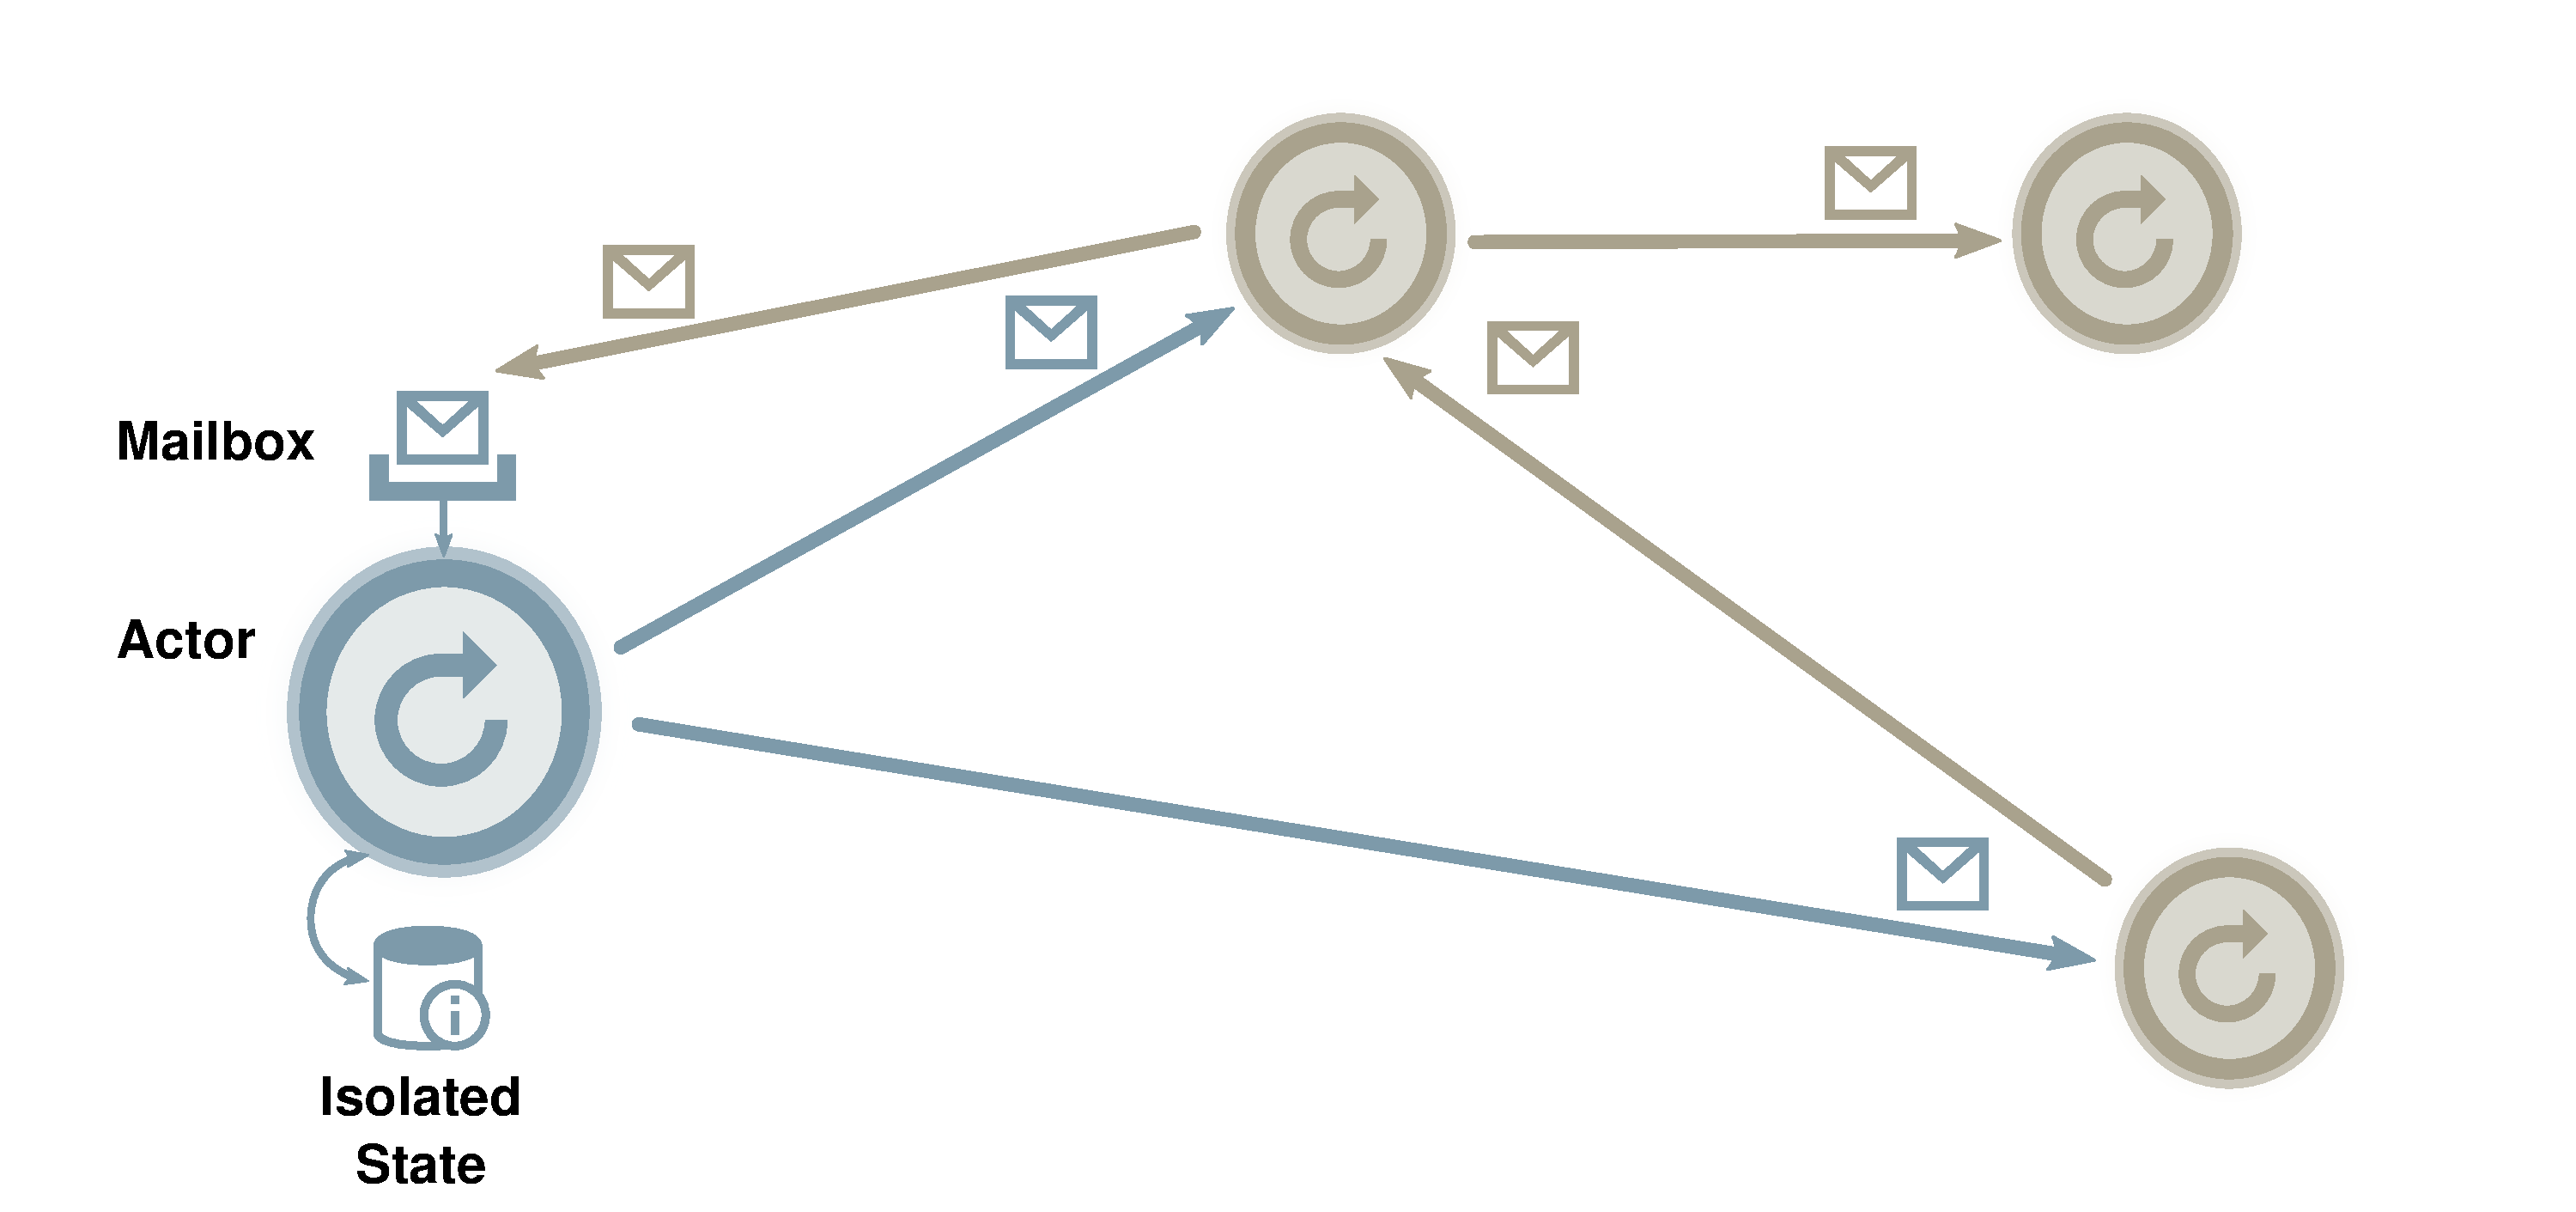
\includegraphics[width=\textwidth]{Images/actors.pdf}
\end{figure}
\end{frame}

\subsection{Message Passing}
\begin{frame}
  \frametitle{Message Passing}
  \begin{itemize}
    \item Afsendelse
    \begin{itemize}
      \item Blokerende
      \item Ikke-blokerende
    \end{itemize}
    \item Modtagelse
  \end{itemize}
\end{frame}

%Terndrup
\section{Compiler}

\subsection{F\# Evaluering}
\begin{frame}{F\# evaluering}
  \begin{columns}
    \begin{column}{.5\textwidth}
      \structure{Godt}
      \begin{itemize}
        \item Ny vinkel til programmering
        \item Kort og præcis kode
        \item Exhaustive checks ved pattern matching
      \end{itemize}
    \end{column}
    
    \begin{column}{.5\textwidth}
      \structure{Dårligt}
      \begin{itemize}
        \item Idiomatisk F\# undgår muteringer => mindre effektiv kode
        \item Nyt sprog at lære
        \item Ikke så meget compiler-læremateriale
      \end{itemize}
    \end{column}
  \end{columns}
\end{frame}

\subsection{Struktur}
\begin{frame}{Struktur}
\centering
\resizebox{1\textwidth}{!}{%
\begin{tikzpicture}[>=latex', node distance = 2cm]
        \tikzset{block/.style= {draw, rectangle, align=center,minimum width=1cm,minimum height=1cm},
        input/.style={ % requires library shapes.geometric
        draw,
        trapezium,
        trapezium left angle=60,
        trapezium right angle=120,
        minimum width=1cm,
        align=center,
        minimum height=0.5cm
    },
        }
        \node [coordinate]  (input) {};
        \node [block, right =1cm of input] (parser) {Parser};
        \node [block, above =1cm of parser] (parserErrors) {Errors};
        \node [block, right =2cm of parser] (toAST) {To AST};
        \node [block, right =1cm of toAST] (reass) {Reassignment check};
        \node [block, below =1cm of reass] (usebeforedecl) {Use before declared check};
        \node [block, left =2.2cm of usebeforedecl] (hiding) {Hiding check};
        \node [block, left =2.2cm of hiding] (typecheck) {Typecheck};
        \node [block, above =1cm of reass] (analyserErrors) {Errors};
        \node [block, below =1cm of typecheck] (codegen) {Code generator};
        \node [block, right =1.5cm of codegen] (clang) {Clang};
        \node [coordinate, right =2cm of clang] (nativeCode) {};
%% paths
        \path[draw,->] (input) edge node[anchor=south] {Input} (parser)
                    (parser) edge node[anchor=south] {Hime AST} (toAST)
                    (parser) edge (parserErrors)
                    (toAST) edge node[anchor=south] {AST} (reass)
                    (reass) edge node[anchor=west] {Symbol table} (usebeforedecl)
                    (usebeforedecl) edge node[anchor=north] {Symbol table} (hiding)
                    (hiding) edge node[anchor=north] {Symbol table} (typecheck)
                    (reass) edge (analyserErrors)
                    (typecheck) edge node[anchor=west] {AST} (codegen)
                    (codegen) edge node[anchor=south] {LLVM IR} (clang)
                    (clang) edge node[anchor=south] {Native Code} (nativeCode)
                    ;
       \path[draw, ->] (toAST) [dashed] edge (usebeforedecl)
                       (toAST) [dashed] edge (hiding)
                       (toAST) [dashed] edge (typecheck);
    \end{tikzpicture}
    }

\end{frame}

\subsection{Overgang Mellem Faser}
\begin{frame}[fragile]
  \frametitle{Overgang Mellem Faser}
  \begin{lstlisting}[language=fsharp]
parse input grammarPath 
>>= fun tree -> Success (toAST tree)
>>= analyse
>>= (fun ast -> Success (codeGen ast))
  \end{lstlisting}

  \begin{lstlisting}[language=fsharp]
let parse (srcInput:string) (grammarPath:string) : Result<ASTNode> = ...
  \end{lstlisting}

  \begin{lstlisting}[language=fsharp]
let rec toAST (root:ASTNode) : AST = ...
  \end{lstlisting}

  \begin{lstlisting}[language=fsharp]
type Result<'a> =
     | Success of 'a
     | Failure of string list
  \end{lstlisting}

  \begin{lstlisting}[language=fsharp]
let (>>=) (res:Result<'a>) (f:'a -> Result<'b>) : Result<'b> =
    match res with
    | Success r -> f r
    | Failure errs -> Failure errs
  \end{lstlisting}

  

\end{frame}

\subsection{Alternativ Compiler Struktur}
\begin{frame}{Alternativ Compiler Struktur}
  \begin{itemize}
    \item Dekorere AST igennem faser => undgå symbol tabel
    \item Mere uafhængig struktur => alting er transformationer
  \end{itemize}
\resizebox{1\textwidth}{!}{%
\begin{tikzpicture}[>=latex', node distance = 2cm]
        \tikzset{block/.style= {draw, rectangle, align=center,minimum width=1cm,minimum height=1cm},
        input/.style={ % requires library shapes.geometric
        draw,
        trapezium,
        trapezium left angle=60,
        trapezium right angle=120,
        minimum width=1cm,
        align=center,
        minimum height=0.5cm
    },
        }
        \node [coordinate]  (input) {};
        \node [block, right =1cm of input] (parser) {Parser};
        \node [block, above =1cm of parser] (parserErrors) {Errors};
        \node [block, right =2cm of parser] (toAST) {To AST};
        \node [block, right =1cm of toAST] (reass) {Reassignment check};
        \node [block, below =1cm of reass] (usebeforedecl) {Use before declared check};
        \node [block, left =2.4cm of usebeforedecl] (hiding) {Hiding check};
        \node [block, left =2.4cm of hiding] (typecheck) {Typecheck};
        \node [block, above =1cm of reass] (analyserErrors) {Errors};
        \node [block, below =1cm of typecheck] (codegen) {Code generator};
        \node [block, right =1.5cm of codegen] (clang) {Clang};
        \node [coordinate, right =2cm of clang] (nativeCode) {};
%% paths
        \path[draw,->] (input) edge node[anchor=south] {Input} (parser)
                    (parser) edge node[anchor=south] {Hime AST} (toAST)
                    (parser) edge (parserErrors)
                    (toAST) edge node[anchor=south] {AST} (reass)
                    (reass) edge node[anchor=west] {Decorated AST} (usebeforedecl)
                    (usebeforedecl) edge node[anchor=south] {Decorated AST} (hiding)
                    (hiding) edge node[anchor=south] {Decorated AST} (typecheck)
                    (reass) edge (analyserErrors)
                    (typecheck) edge node[anchor=west] {Decorated AST} (codegen)
                    (codegen) edge node[anchor=south] {LLVM IR} (clang)
                    (clang) edge node[anchor=south] {Native Code} (nativeCode)
                    ;
    \end{tikzpicture}
    }

\end{frame}
\section{Konkret Sprog Design}
\setlength{\grammarindent}{100pt}
\subsection{Expressions}
\begin{frame}
	\frametitle{Expressions - Grammatik}
	\dots
	\begin{grammar}
	<OP2> ::= <OP2> <Poneoperator> <OP1>
  \alt <OP1>
  
	<OP1> ::= <Pzerooperator> <OP1>
  \alt <OP0>

  <OP0> ::= <Operand>
  \alt '(' <Expression> ')'
  \end{grammar}
	\dots
	\begin{grammar}
	<PTWOOPERATOR> ::= '*' | '/' | '\%'
	
	<PTHREEOPERATOR> ::= '+' | '-'
	
	<PFOUROPERATOR> ::= '=' | '!=' | '$\textless$' | '$\textless$=' | '$\textgreater$' | '$\textgreater$='
	\end{grammar}
	\dots
\end{frame}

\begin{frame}
	\frametitle{Expressions - Grammatik}
	\begin{grammar}
  <Operand> ::= <Integer>
    \alt <Real>
    \alt <Boolean>
    \alt <Invocation>
    \alt <Literals>
		\alt <Block>
  \end{grammar}
\end{frame}

\begin{frame}
	\frametitle{Expressions - Grammatik}
	\begin{grammar}
  <Operand> ::= <Integer>
    \alt <Real>
    \alt <Boolean>
    \alt <Invocation>
    \alt <Literals>
		\alt <Block>
		
	<Literals> ::= <String>
    \alt <Char>
    \alt <List>
    \alt <StructLiteral>
    \alt <Tuple>
  \end{grammar}
\end{frame}

\subsection{Typesystem}
\begin{frame}
	\frametitle{Typesystem - Block}
	\begin{align*}
  &\inference[BLOCK]{\Tenv s_1: \Tt & \Tenv s_2: \Tt'}
                    {\Tenv \{s_1; s_2\} : \Tt'}
	\\\\
  &\inference[BLOCK]{\Tenv s_1: \Tt & \Tenv s_2: \Tt' & \Tenv s_3: \Tt''}
                    {\Tenv \{s_1; \;\Treturn\; s_2; s_3\} : \Tt'}
  \end{align*}
\end{frame}

\subsection{Statements}
\begin{frame}
  \frametitle{Statements - Grammartik}
	\begin{grammar}
  <Statement> ::= <Declaration>
    \alt <Reassignment>
    \alt <Expression>
    \alt <Receive>
    \alt <Spawn>
    \alt <Return>
    \alt <Die>
    \alt <Send>
    \alt <If>
    \alt <IfElse>
    \alt <While>
    \alt <ForIn>
  \end{grammar}
\end{frame}

\subsection{Semantik}
\begin{frame}
	\frametitle{Semantik - Transitions System}
	\begin{center}	
  $at = \text{ActorTypes} \rightharpoonup \text{Stm}$
	
	$aEnv = \text{Anames} \cup {next} \rightharpoonup sEnv$
	
	$sEnv = \text{Symbols} \rightharpoonup \text{Stm} \times \text{Symbols}$
  \end{center}
\end{frame}

\begin{frame}
	\frametitle{Semantik - Invoke}
	\begin{align*}
	&\inference[$\text{INVOKE}_{A}$]{}
                  {\Braket{x,aEnv,sEnv} \Rightarrow_A v}
                  \\
									&{,aEnv,sEnv(x) = \Braket{n,\epsilon}, \mathcal{N}(n) = v}
	\\\\
	&\inference[$\text{INVOKE}_{B\top}$]{}
                  {\Braket{x,aEnv,sEnv} \Rightarrow_A \top}
                  {,sEnv(x) = \Braket{true,\epsilon}}
	\\\\
	&\inference[$\text{INVOKE}_{B\bot}$]{}
                  {\Braket{x,aEnv,sEnv} \Rightarrow_A \bot}
                  {,sEnv(x) = \Braket{false,\epsilon}}
	\end{align*}
\end{frame}

\begin{frame}
  \frametitle{Semantik - Invoke}
  \begin{align*}
	&\inference[$\text{INVOKE}_{S1}$]{}
                  {\Braket{x,aEnv,sEnv} \Rightarrow_A \Braket{\{S\},s}}
									\\
                  &{sEnv(x) = \Braket{\{S\},s}}
	\\\\
	&\inference[$\text{INVOKE}_{S2}$]{}
                  {\Braket{x(),aEnv,sEnv} \Rightarrow_A \Braket{\{S\},aEnv,sEnv}}
									\\
                  &{sEnv(x) = \Braket{\{S\},\epsilon}}
	\\\\
	&\inference[$\text{INVOKE}_{S3}$]{}
                  {\Braket{x(y),aEnv,sEnv} \Rightarrow_A \Braket{\{S_1\},aEnv,sEnv[z \mapsto \Braket{S_2,s}]}}
                  \\
					        &{sEnv(x) = \Braket{\{S_1\},z}, sEnv(y) = \Braket{S_2,s}}
	\end{align*}
\end{frame}
%Aloxander
%Heider

\end{document}
\section{Message Passing Interface}
Message Passing Interface (MPI) is the de facto standard for message passing, when doing high performance computation. It was first released in 1994 as version 1.0. It was created in collaboration between 40 different organisations involving about 60 people in total. It was based in a preliminary proposal, known as MPI1, that was created by Jack Dongarra, Rolf Hempel, Tony Hey, and David Walker and finished in November 1992 and inspired from the, then, state of the art practice, such as PVM, NX, Express, p4, etc. It has since been iterated upon, with the latest version, MPI-3.0 being released in 2012.

The reason for creating this standard is to ensure portability and ease-of-use. In a communicating distributed memory environment, high-level routines and abstractions are often build upon lower level message passing routines, of which this standardisation ensures that these abstractions and routines are available on all systems. This also presents vendors with a few clearly defined base-routines they need to implement efficiently and, if possible, provide hardware support for, to enhance scalability.

MPI is designed to allow efficient communication between processes, use in heterogeneous environments and ensure thread-safety. The semantics of the interface itself should be independent from any language it is implemented in, however it does focus on providing convenient bindings for the C and Fortran languages. MPI also specifies how communication failures are dealt with, in the underlying systems.

The standard is designed for message passing only and does not include specifications for explicit operations on shared memory. Operations, that go beyond the current operating system support, are not included. These include interrupt-driven receives, remote execution and active messages, since the interface is not intended for kernel programming/embedded systems. Neither does it include support for debugging, explicit support for threads or task management nor support for I/O functions.

(Source: http://www.mpi-forum.org/docs/mpi-1.0/mpi-10.ps chapter 1)

\subsection{Message Types}

\subsubsection{Point-to-point Operations}
Point-to-point communication is the the basic building block of message passing.
\paragraph{Send}
Here one process sends data in form of a message to a single other process.
\paragraph{Receive}
When a process receives a message, it enqueues the message in a queue called its message box. Each message in the message box is processed sequentially by dequeuing and handling them one at a time.

(Source: http://www.mpi-forum.org/docs/mpi-1.0/mpi-10.ps chapter 3)

\subsubsection{Collective Operations}
\paragraph{Broadcast}
Broadcast is a one-to-many operation, where one process has some specific data that it sends to many other processes. The data is therefore multiplied, as opposed to being divided.

\paragraph{Scatter}
Scatter is a close relative to broadcast. It is also a one-to-many operation, but here the data is divided into equally large chunks and is distributed among multiple processes (including the process originally containing all the data). This could for instance be sending all entries in a collection to different processes that individually process their part.

\paragraph{Gather}
Gather is a many-to-one operation and is the inverse of scatter. Here data from many processes are sent to one of them. This operation often implies a hierarchy of the processes containing the data, where the process highest in the hierarchy receives all the data (also from itself).

\paragraph{Reduce}
Reduce is a many-to-one operation. Here one operation, called the reduction function, is done on data from multiple processes and the result is placed in one of them. As with gather, a hierarchy is also customary and the process highest in the hierarchy receives the result of the reduction. All reduction functions must be both associative and commutative, so results can be reduced without concern for the order of operations.
(Source: http://www.mpi-forum.org/docs/mpi-1.0/mpi-10.ps chapter 4)

\subsubsection{System Buffer}
Consider the following: When sending messages, what happens if the receiver is not ready to process them? To solve this problem, MPI dictates that an implementation must be able to store messages, however the way this is done is up to the implementer.

One way to do this is with a system buffer. In short terms, a system buffer works as an inbox, and sometimes also an outbox, where messages are stored until they can be processed. A few things to note about this inbox, is that it is supposed to work "behind the scenes", not manageable by the programmer. However, what the programmer needs to realise, is that this buffer is a finite resource, which will be exhausted if one is not cautious.
(Source: MPI\_tut1)

\subsubsection{Blocking and Non-blocking Sends}
Messages can be divided into two distinct groups, the blocking sends and the non-blocking sends. The straight forward approach is the non-blocking send, where the sender assumes, or is certain, that the receiver is ready to handle the message. These types of messages return almost immediately, but there is no guarantee that the message was received, or how it was received.

On the other hand there is the blocking send. This only returns after it is safe to modify the application buffer again. The sent data could still be sitting in a buffer, but it is considered safe.

Generally, blocking sends are used for cases where it is crucial that the communication has been completed, and non-blocking sends are used to increase performance in cases where the communication is not crucial.
(Source: MPI\_tut2)

\subsubsection{Order and Fairness}
When sending messages, the order in which they are sent and received can matter a great deal. MPI gives a few guarantees as to how this can be expected to happen. One must note that these rules are not enforced if multiple threads are participating in the communication.

When using MPI, messages will not overtake each other. If one task sends out two messages in succession, the message sent out first, will be the first one to be received. Also, if a receiver has multiple requests looking for a matching message, the request that was made first, will get the first match.

MPI does not give any guarantees related to fairness. It is entirely possible to starve tasks. If this is not desired, the responsibility lies with the programmer.
(Source: MPI\_tut3)

\chapter{The Actor Model}
The actor model is a concurrency model, which first appeared in 1973 in the report "A Universal Modular ACTOR Formalism for Artificial Intelligence" by Carl Hewitt, Peter Bishop and Richard Steiger [worrydream.com/refs/Hewitt-ActorModel.pdf]. This chapter will explain the model generally. In addition to the general model, the model will be compared to alternative concurrency models and a few implementations of the model will be briefly described.

\section{Model}
The actor model is focused on the fact that any computational behaviour, be it functions, processes or data structures, can be modelled as a single behaviour; sending messages to actors.
An actor in this context is a process, which has its own isolated state, used to store values and modify its own behaviour, and a message box, for receiving messages. An actor can only share information by sending messages, asynchronously, to other actors. 
Actors are very similar to the communicating sequential processes (CSP) described in C.A.R. Hoare's publication "Communicating Sequential Processes". Actors, though, have a few well-defined behaviours in response to receiving a message, where CSPs are free to exhibit other behaviour. An actor can, in response to a message: 
\begin{enumerate}
  \item Send a finite number of messages to other actors.
  \item Spawn a finite number of new actors.
  \item Change its own behaviour for the next message that is received.
\end{enumerate}

In figure \ref{fig:actor}, a model of an actor based program can be seen.

\begin{figure}
  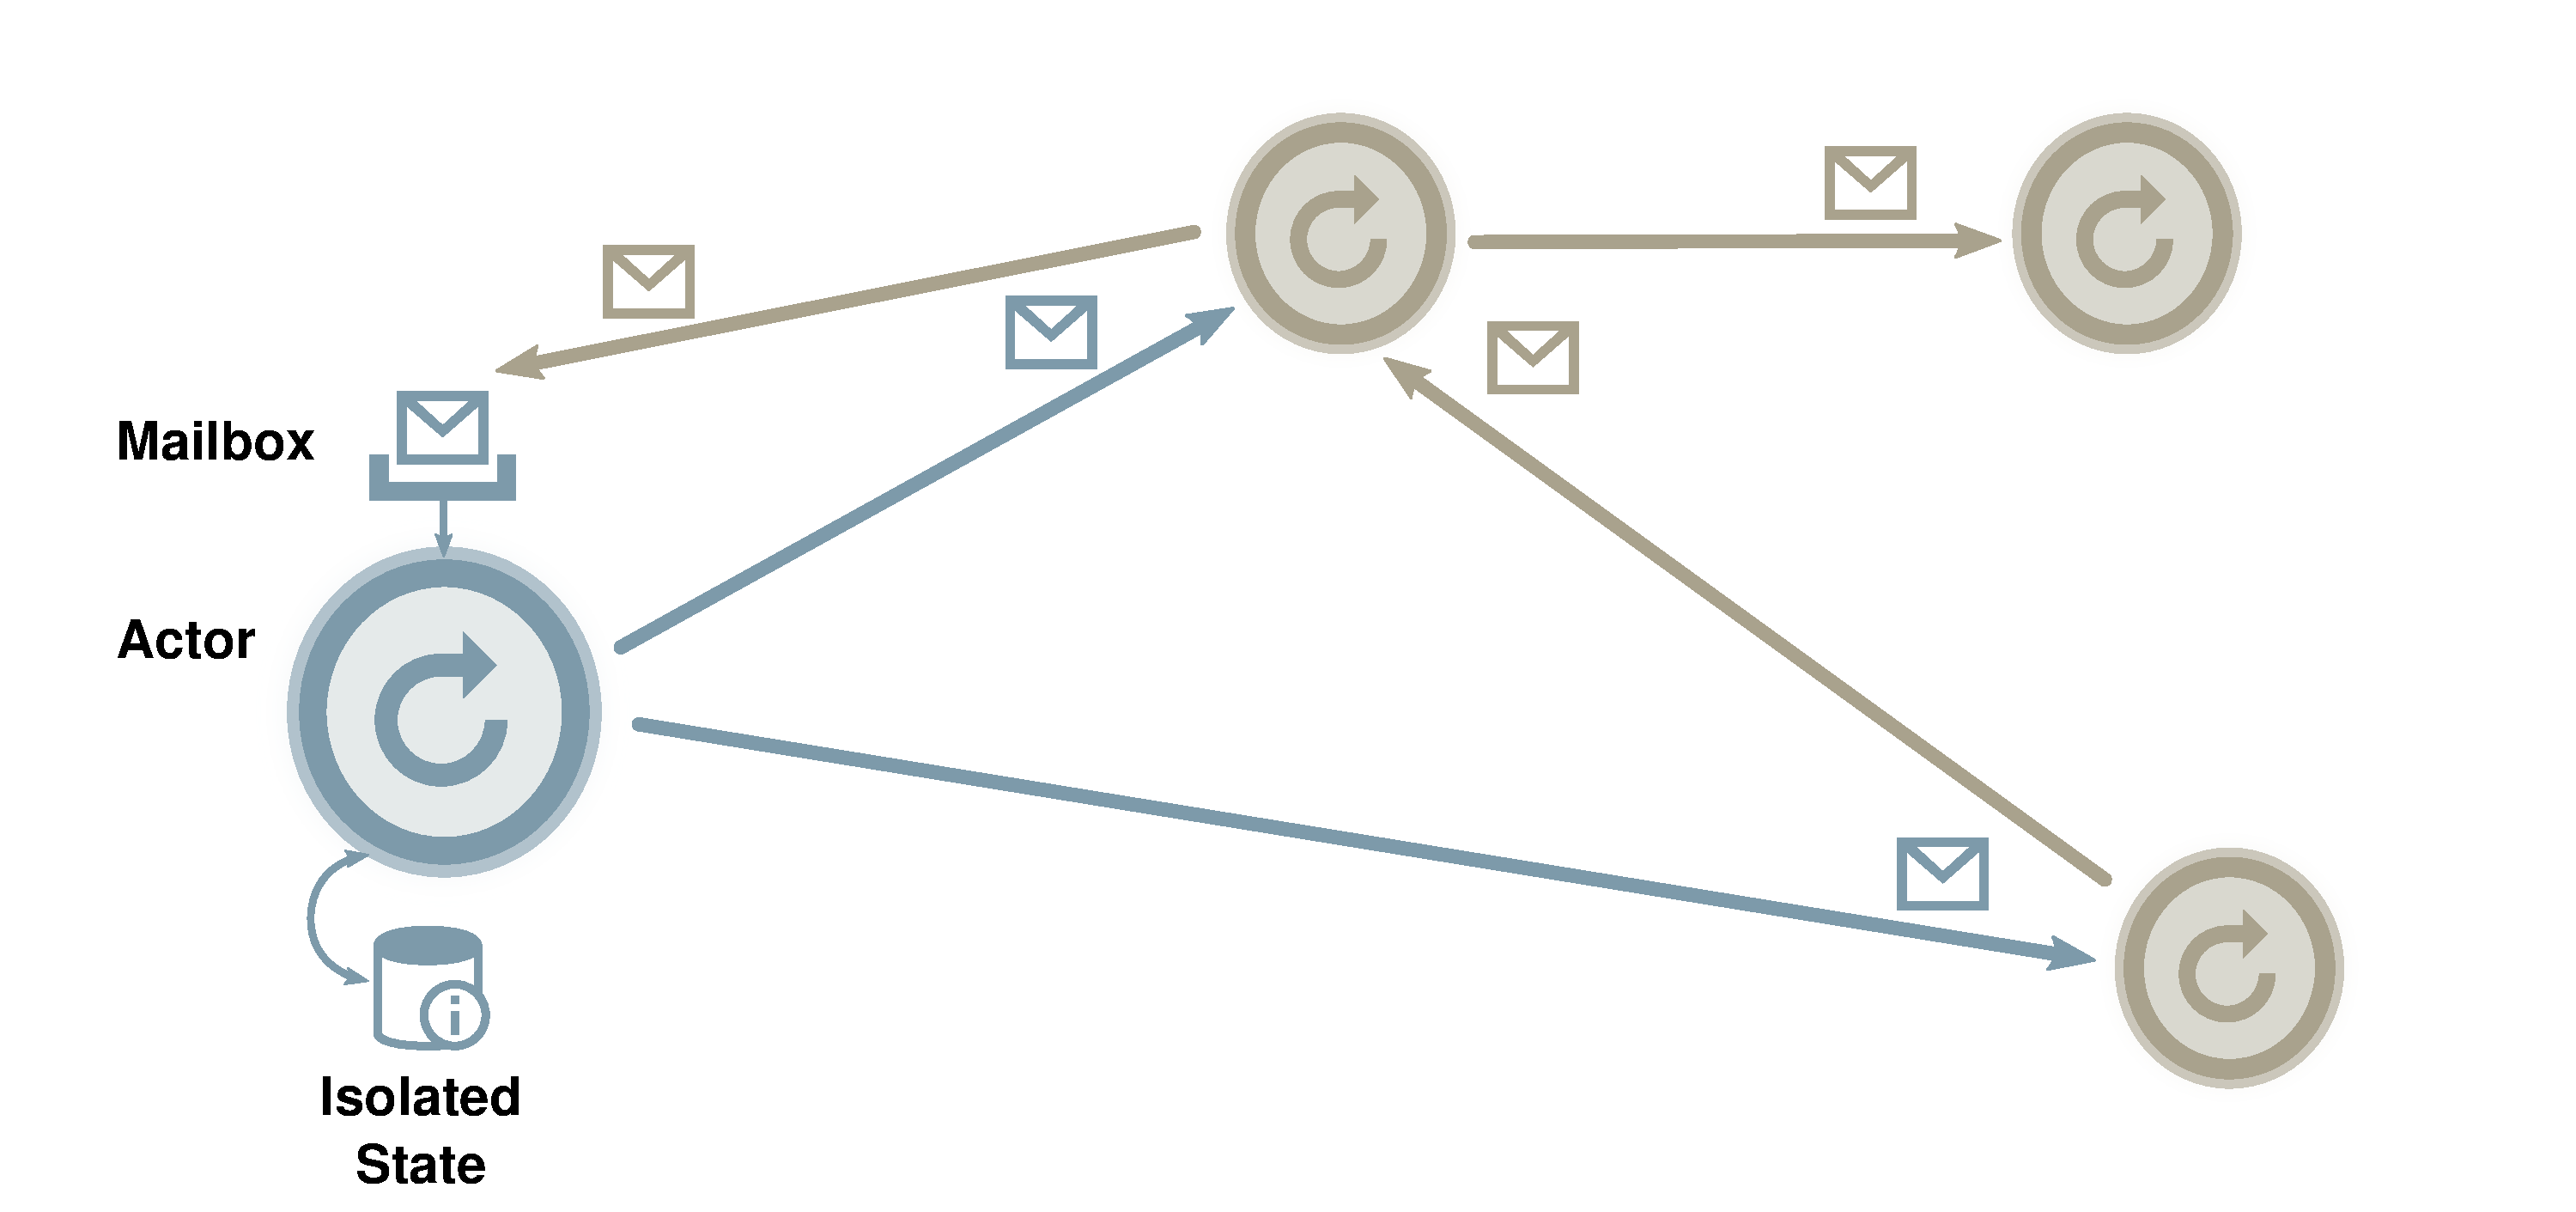
\includegraphics[width=\textwidth]{Images/actors.pdf}
  \caption{A model of an example program using actors. The nodes in this graph represent actors and the edges represent messages being sent.}
  \label{fig:actor}
\end{figure}


\subsection{Adding Logic}
One of the main features of the actor model is, as Hoare describes it, the ability to add knowledge to a system, without rewriting the existing knowledge. This means that if a developer is interested in adding a logical step in the business logic of his system, this can be achieved by merely adding an actor, which can perform the logical operations, that are to be added, and then adding that actor as a link in the flow of logic.

\subsubsection{Example}
We have a system which can read a CSV-file and print it to stdout. This can be implemented using actors in the following way:\\
let Reader and Printer be actors.

\begin{tabular}{ | c | c | c | }
\hline
Step & Reader & Printer \\\hline
1 & \textbf{Read CSV-file} & \textit{Wait for message} \\\hline
2 & \textbf{Send data to Printer} & \textit{Wait for message}\\\hline
3 & \textit{Wait for message} & \textbf{Receive data from Reader}\\\hline
4 & \textit{Wait for message} & \textbf{Print data to stdout}\\\hline
\end{tabular}\\
At som point we decide that we wish to format our data before printing it. To do so, we create and incorporate a new actor, Formatter, which changes the flow of execution in this manner:

\begin{tabular}{ | c | c | c | c | }
\hline
Step & Reader & Formatter & Printer \\\hline
1 & \textbf{Read CSV-file} & \textit{Wait for message} & \textit{Wait for message} \\\hline
2 & \textbf{Send data to Formatter} & \textit{Wait for message} & \textit{Wait for message}\\\hline
3 & \textit{Wait for message} & \textbf{Receive data} & \textit{Wait for message} \\\hline
4 & \textit{Wait for message} & \textbf{Format data} & \textit{Wait for message} \\\hline
5 & \textit{Wait for message} & \textbf{Send data to Printer} & \textit{Wait for message} \\\hline
6 & \textit{Wait for message} & \textit{Wait for message} & \textbf{Receive data}\\\hline
7 & \textit{Wait for message} & \textit{Wait for message} & \textbf{Print data to stdout} \\\hline
\end{tabular}\\

Notice that in adding the new logic, the only existing logic that was changed is the actor whom Reader sends data to.

\subsection{Supervisors}
Most implementations of the actor model implement a form of a supervisor-worker relationship. This means that every actor has a supervisor, typically their parent, to whom they report failures. The supervisor then has to deal with the failure, by for example restarting the failed actor.
Supervisors in the actor model works very well with the "fail fast"-principle of programming, meaning, in the actor model, that an actor will not try to continue operation or correct an error when encountering a failure. An actor that has failed will, as soon as the failure is detected, report the failure to its supervisor and halt operation, moving the responsibility of handling the failure up the supervision tree.

\section{Implementations}
\subsection{Erlang}
When talking about the actor model, one cannot escape the subject of Erlang. Erlang is one of first languages to fully incorporate the actor model as the main model of concurrency. Erlang is a purely functional language, developed for the telecommunications industry, where a lot of concurrent processes have to be handled. 
Actors in Erlang, or processes as they are called, are controlled by a few very simple constructs; actors can be spawned using the built-in spawn-function, the spawn-function takes three arguments, the module in which the actor is contained, the function that defines the behaviour for the actor and an initial message. You can send messages to actors using the bang-operator (!) and you can define an actor's behaviour in a receive-block.
In Erlang, an actor's parent is it's supervisor, if one chooses to use the supervisor module available. Using the supervisor module in Erlang gives the programmer the ability to choose different strategies to be used when a child actor fails. These strategies are:
\begin{enumerate}
  \item Respawn the failed child
  \item Respawn all children when one fails
  \item Respawn all children after the child in the start order of the children
\end{enumerate}

\subsubsection{Using actors in Erlang - Example}
To demonstrate the use of actors in Erlang, a simple example is shown in listing \ref{lst:ErlExample}. This program has only one actor, which counts the number of "incr"-messages it has been sent.

\begin{lstlisting}[style=erlang, caption={A simple message-counter in Erlang.}, label=lst:ErlExample]
-module(countMsgs).
-export([run/0, counter/1]).

run() ->
  S = spawn(countMsgs, counter, [0]), %spawn S as counter-actor
  sendMsgs(S, 10000), %send 10000 messages to S
  S.
  
counter(Sum) -> %function-definition for counter-actor
  receive
    value -> io:fwrite("Value is ~w~n", [Sum]);
    incr -> counter(Sum+1)
  end.

sendMsgs(_, 0) -> true; %base case
sendMsgs(S, N) -> %recursive function to send N messages to actor S
  S ! incr, %send incr to S
  sendMsgs(S, N-1).
\end{lstlisting}

\subsection{Akka}
A more modern approach to the actor model is taken in Akka, a concurrency toolkit for Scala and Java.
In Akka, an actor is just an object, which extends Akka's Actor-class and implements a receive method. One difference in the receive-method from Erlang's receive-block is that Akka's receive-method is exhaustive, meaning that the programmer has to define behaviour for all possible messages that an actor can receive. 
Creating an actor in Akka is done by calling the actorOf-method, on an actor or an instance of ActorSystem, which acts as the parent of top-level actors. The actorOf-method takes a Probs as an argument, Probs is just an object containing properties for an actor, such as the definition of the actor. Just like Erlang, messages are sent using the bang-operator.
In Akka, supervisors have the ability to handle failures in child actors in the following manner:
\begin{enumerate}
  \item Ignore failure and resume operation
  \item Restart the child from initial state
  \item Terminate the child, without respawning it
  \item Fail (move failure up supervision tree)
\end{enumerate}

\subsubsection{Using Actors in Akka - Example}
To demonstrate Akka's implementation of actors, the same example shown in listing \ref{lst:ErlExample} will be implemented in Scala, using Akka, in listing \ref{lst:AkkExample}.


\begin{lstlisting}[style = scala, caption={A simple message-counter in Scala.}, label=lst:AkkExample]

import akka.actor.Actor
import akka.actor.Probs

class Counter extends Actor{ //definition of counter-actor
  var count = 0
  def receive = {
    case "incr" => count += 1 //if actor receives "incr", increment count
    case "value" => println(s"Value is $count")
    case other => println(s"Error: Cannot understand message $other") //default case
  }
}

object Main extends App {
  val mySystem = ActorSystem("MySystem")
  val myCounter = mySystem.actorOf(Probs[Counter], name="MyCounter") //create counter-actor as top-level actor
  def main(args:Array[String]){
    for (i <- 1 to 10000) { //send 10000 messages to myCounter
      myCounter ! "incr"
    }
  }
}
\end{lstlisting}


\section{Criteria for Language Design}\label{analsum}

This section will, in light of the preceding two chapters, \cref{part:analysis} and \cref{part:analysis2}, settle on some criteria for TLDR. The criteria are inspired by those found in \cite{sebesta2015concepts}. However, only those characteristics which differentiate TLDR will be discussed, even though other characteristics will be present in the language.


\subsection{Simplicity, Orthogonality and Syntax Design}

In order to accommodate a user group with programming as secondary skill sets, TLDR should be simple. This would result in strict and straightforward rules regarding interactions. The language should try to keep simple rules regarding orthogonality as well, but not necessarily be highly orthogonal for that reason. One such rule, based on properties of the actor model, is that actors should, in the eyes of the programmer, only communicate through messages either sent or received. This would prohibit directly addressing fields in an actor, which would lower orthogonality, but keep the language simple. The syntax design, should for the same reasons, cater towards a modelling perspective and not necessarily a technical accurate perspective.

\subsection{Data Types}

Since the users of TLDR are will typically have a background in mathematics, or require to include some mathematics in order to asses the value of any given result of a simulation, the language should strive towards having data types which allow for representation of traditional mathematical numbers.


\subsection{Type Checking and Exception Handling}

Due to the language targeting high performance computation, the language should try to avoid run-time errors, and catch problems as early as possible. This suggests a strongly typed language, but we will elaborate further on this matter in \cref{typesys}. For the same reasons, the language will not value exception handling, since edge cases should be fully encompassed in a simulation. However it is worth noticing that the actor model could require exception handling, if communication problems, caused by either race conditions or network conditions, should prove frequent.


%\subsection{Support for abstraction}


%\subsection{Aliasing}
